\documentclass[11pt, a4paper]{article}
\usepackage{amsmath, amsthm, amssymb, calrsfs, wasysym, verbatim, bbm, color, graphics, geometry}
\usepackage[utf8]{inputenc} % comment when using lualatex
\usepackage[italian]{babel} % lingua e a-capo-sillabato
\usepackage{fullpage}
\usepackage{graphicx}
%\usepackage[hidelinks]{hyperref,xcolor} % link di pagina
\usepackage[bottom]{footmisc} % note appiccicate al fondo della pagina
\usepackage{float} % per posizionamento immagini
\usepackage{cancel}

\geometry{tmargin=.75in, bmargin=.75in, lmargin=.75in, rmargin = .75in}  

\newcommand{\R}{\mathbb{R}}
\newcommand{\C}{\mathbb{C}}
\newcommand{\Z}{\mathbb{Z}}
\newcommand{\N}{\mathbb{N}}
\newcommand{\Q}{\mathbb{Q}}
\newcommand{\Cdot}{\boldsymbol{\cdot}}

\newtheorem{thm}{Theorem}
\newtheorem{defn}{Definition}
\newtheorem{conv}{Convention}
\newtheorem{rem}{Remark}
\newtheorem{lem}{Lemma}
\newtheorem{cor}{Corollary}



\definecolor{dkgreen}{rgb}{0,0.6,0}
\definecolor{gray}{rgb}{0.5,0.5,0.5}
\definecolor{mauve}{rgb}{0.58,0,0.82}


\title{Distributed Systems}
\author{Raffaele Castagna}

\date{Academic Year 2025-2026}

\begin{document}

\maketitle

\tableofcontents
\newpage

\section{Introduction}
\begin{defn}
    In a system we have \textit{n} processes in $\prod:{p_{0}\dots,p_{n-1}}$ each with a distinct identity
    they communicate by utilizing a communication graph \textbf{G : ($\prod,E$)}, the communication is done by exchanging messages.

\end{defn}
\begin{center}
    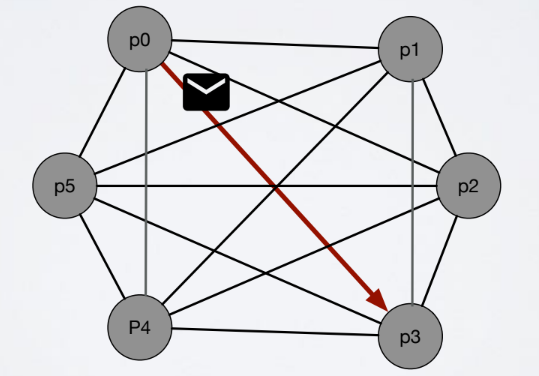
\includegraphics[scale=0.6]{img/comm graph}
\end{center}
\begin{defn}
A process is a (possibily infinite) State Machine (I/O Automaton).
\end{defn}
\begin{center}
    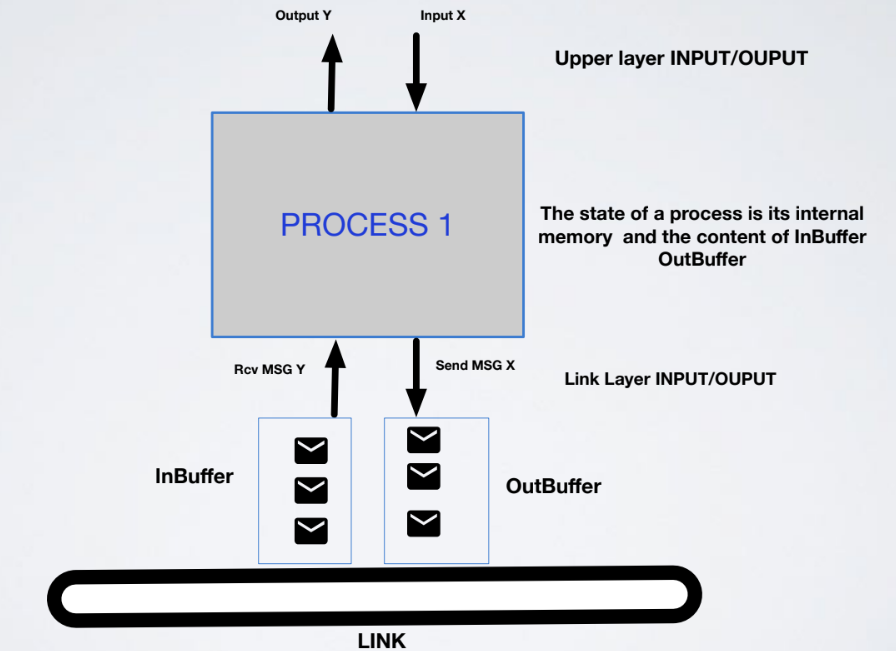
\includegraphics[scale=0.55]{img/process.png}
\end{center}
Each process has multiple qualities:
\begin{itemize}
    \item A set of internal states \textit{Q}
    \item A set of initial states $Q_i \subset Q$
    \item A set of all possible messages M in the form <sender,receiver,payload>
    \item Multiset of delivered messages $InBuf_j$
    \item Multiset of inflight messages $OutBuf_j$
\end{itemize}
\newpage
We can formally describe this as follows: (this isnt part of the exam btw) 
$$P_j (q \in Q \cup Q_{in},InBuf_j) = (q' \in Q, SendMsg \subset M \newline)$$  $$ OutBuf_j = OutBuf_j \cup SendMsg$$ $$\newline InBuf_j = \cancel{0}$$
To execute a process we have an adversary that schedules a set of events (scheduler), these events may be for example a delivery (e.g. Del(m,i,j)) or it can be one step of the step machine of process i (Exec(i))
\begin{defn}
    A configuration $C_t$ is a vector of n components, component j indicates the state of process j.
\end{defn}
\begin{center}
    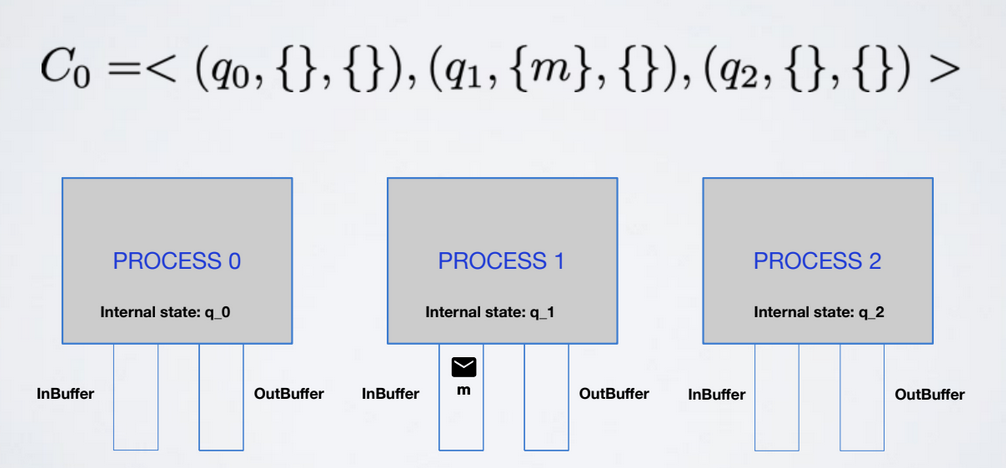
\includegraphics[scale=0.55]{img/configuration.png}
\end{center}
An event is \textbf{enabled} in configuration c if it can happen.
\begin{defn}
    An execution is an infinite sequence that alternates configurations and events: $(C_0,e_0,C_1,e_1,C_2,e_2,\dots)$ such that each event $e_t$ is enabled in configuration $C_t$ and $C_t$ is obtained by applying $e_{t-1} \text{ to } C_{t-1}$

\end{defn}
It may be useful to visualize how an execution involving multiple processes works, here we have an example:
\begin{center}
    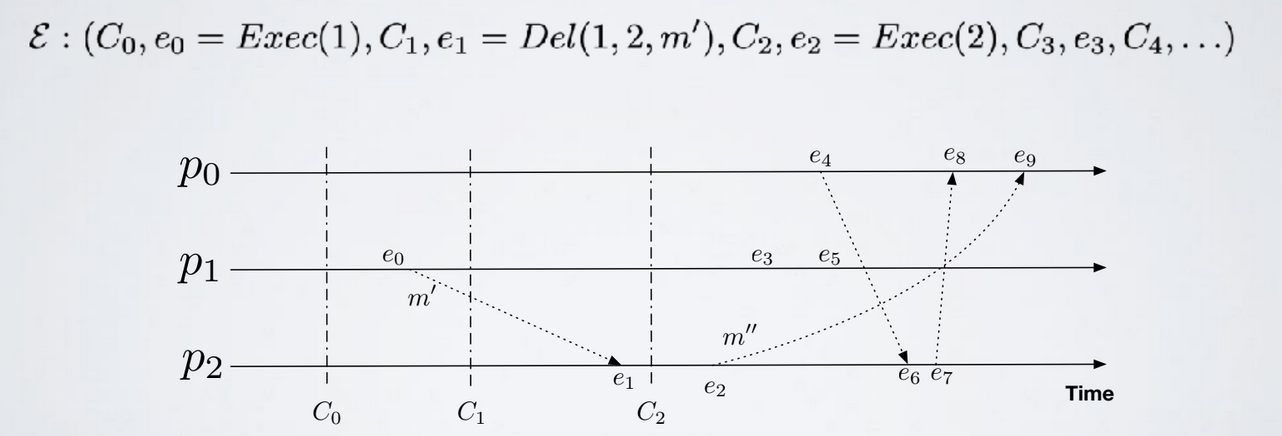
\includegraphics[scale=0.5]{img/execgraph.png}
\end{center}
\newpage
\begin{defn}
    A \textbf{fair execution} is an execution E where each process $p_i$ executes an infinite number of local computations (Exec(i) events are not finite) and each message m is eventually delivered (we can't stall messages)
\end{defn}
We will always use fair executions unless stated otherwise.
\begin{defn}
    Given an execution E and a procces $p_j$, we define the local view/ local execution of $E|p_j$ the subset of events in E that impact $p_j$
    \begin{center}
        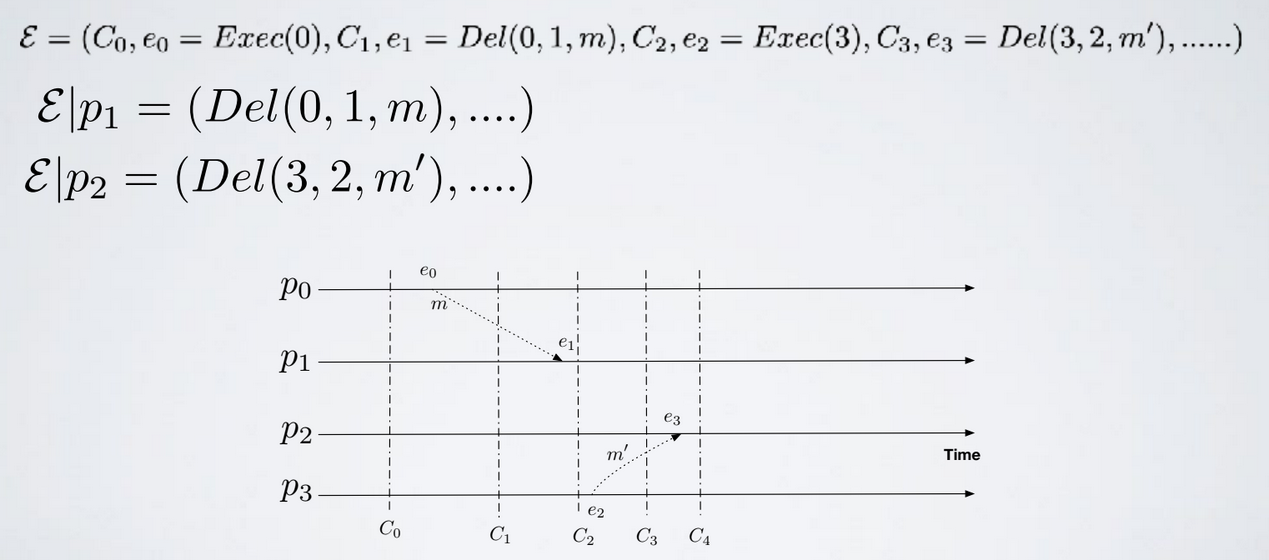
\includegraphics[scale=0.5]{img/localexec.png}
    \end{center}
\end{defn}
But these executions do not account for time, so we may have executions that are the same even though the events happened at different times, in case this does happen, we say that two executions are \textbf{\textit{indistinguishable}}.
\begin{thm}
In the asynch. model there is no distributed algorithm capable of reconstructing the system execution.
\end{thm}

\subsection{Synchronous Vs Asynchronous}
We have 3 main types of synchrony:
\begin{itemize}
    \item Asynchronous Systems
    \item Eventually Synchronous Systems
    \item Synchronous systems
\end{itemize}
We can say that is a system is synchronous if it has a fixed bound on the daly of messages, on the time of actions executed by processes, and a fixed bound between execution of actions.
\subsection{Failures}
We have 2 main models for failures:\\
\begin{itemize}
    \item Crash-stop Failures (The program crashes, and doesnt respond)
    \item Byzantine Failures (The behaviour of the program is random)
\end{itemize}
We signal crash failures with a star sign and byzantile failures with a !
\begin{center}
    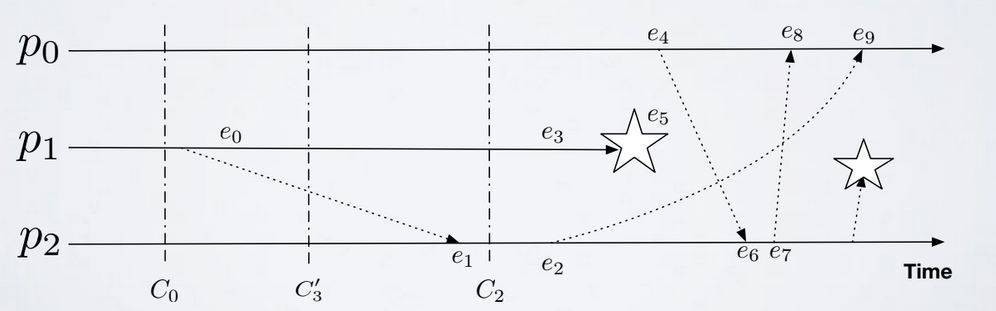
\includegraphics[scale=0.6]{img/crash.png}\\
    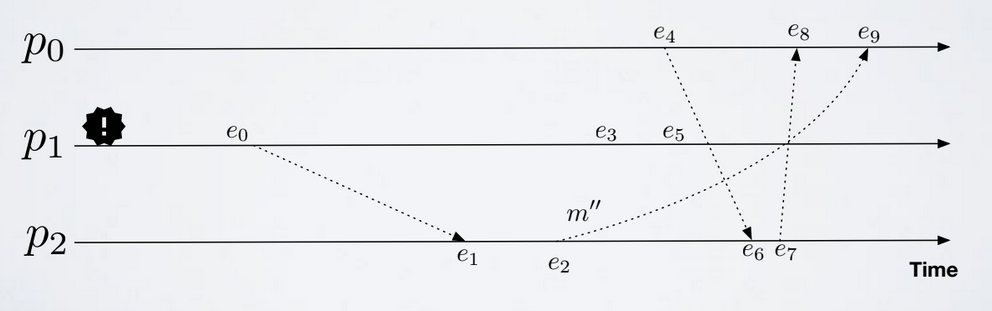
\includegraphics[scale=0.6]{img/byz.png}
\end{center}
Byzantine failures are a superset of Crashstop failures, so algorithms that will work on byzantine failures will always work on crash stop failures, but not the contrary.\\
A process is \textbf{correct} if it does not experience a failure, every algorithm has a maximum number f of failures that i can experience.

\subsection{Different types of links}

\begin{defn}
    An \textbf{Abstraction} is the formalization of a problem/object, to built one we must define the system model and formalize a problem/object so that there is no ambiguity regarding the properties of our abstraction
\end{defn}
For example let us abstract a link: it is something that may lose a message with a certain probability $pr$, the messages can be duplicated a finite number of times and they must come from somewhere.\\
Inside a link we have two main eents:
\begin{itemize}
    \item \textbf{Requests}: $<$Send | q,m$>$ sends message m to process q
    \item \textbf{Indication}: $<$Deliver | p,m$>$ delivers a message m from process p (this might just be an indetifier, e.g. an ip adress or mac address)
\end{itemize}
Now let us formalize this further via its properties:
\begin{itemize}
    \item \textbf{FL1}: (Fair loss) If a correct process p sends infinetely often m, a process q then delivers m an infinite number of times. (e.g. suppose we have $\frac{1}{2}$ probability and we send it over 10 times, then the probability will be $1 - \frac{1}{2^{10}}$ as events are independentm aka if we try hard enough we get the message)
    \item \textbf{FL2}: (Finite duplication) if a correct process p send m a finite number of times to q, then q cannot deliver m an infinite number of times (wel'll receive a finite number of duplicated packets)
    \item \textbf{FL3}: (No creation) If a certain process q sends a message m with send(p),then m was sent by p to q
\end{itemize}
Our objective is hiding the probability behind infinity.\\
A link that respects these properties is called a Fair-lossy link, and its always behind 2 process p and q. We can broadly categorize these properties into two classes:
\begin{itemize}
    \item \textbf{Safety}: if a property is violated at time t, then it cannot be satisfied after that time t. So if in an execution E we violated a safety property, then there is a prefix E' of E such that any extension E' also violates the property, an example of safety property is: if we die, we canno resurrect.
    \item \textbf{Liveness}: these kind of properties cannot be violated in a finite execution, more formally, given an execution E that does not satisfy a liveness property, there is an extension of E that satisfies it, informally it just says that something good will eventually happen.
\end{itemize}
If for example we created a bound on FL2, then we have a safety property, as it cannot be extended, as a rule of thumb, if the property is infinite, then it is a liveness property.\\
Of course there exist badly written properties that try and write both types into a rule, however we should always decompose them (e.g q will eventually deliver and the delivery is unique, if we decompose it we have "q eventually delivers, m is delivered at most once")\\
We also have what we call \textbf{stubborn links}, which inherit FL3 and add:
\begin{itemize}
    \item \textbf{SL1}: (Stubborn delivery) if a correct process p sends m to q, then q delivers m an infinite number of times, hence stubborn.

\end{itemize}
\begin{center}
    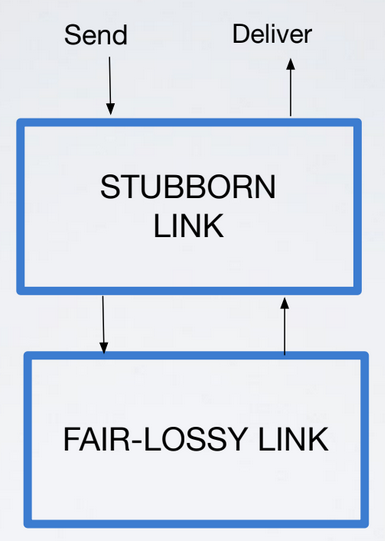
\includegraphics[scale=0.5]{img/links/sl.png}
\end{center}
Our algorithms will always reflect a reactive computing model utilizing handles that consume events or create them, they will always be atomic unless stated otherwise.
\begin{center}
    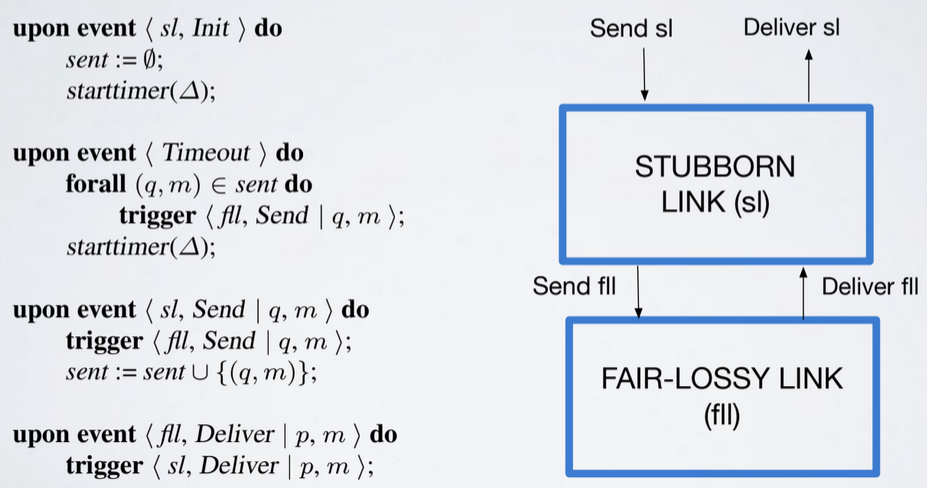
\includegraphics[scale=0.6]{img/links/slalgo.png}
\end{center}
The initialization event creates a set \textit{sent} containing the messages that were sent and then it start a local timer of delta time (delta is whatever we want), we must remember that this timer is not a global clock, but local for that process.\\
In an sl link whenever we get an input we trigger an event to send the message to our fll link, after that we just add it to our set sent.\\
When the fll wants to send a message to a process it will trigger an sl deliver event.\\
When a timeout event happens we scan all the messages in the sent set and we send them again, after that we start a timer.
\\\\
Then we have our \textbf{Perfect P2P} links which inherit FL3 but add the following properties:
\begin{itemize}
    \item \textbf{PL1}: Reliable delivery, if a correct process p sends m to q, then q eventually delivers m
    \item \textbf{PL2}: No duplication, a message is delivered at most once.
\end{itemize}
\begin{center}
    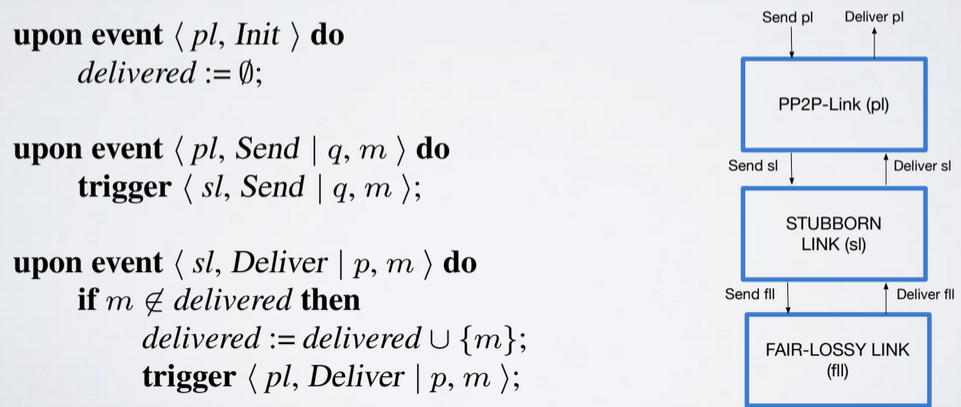
\includegraphics[scale=0.5]{img/links/p2p.png}
\end{center}
We initialize it with a delivered empty set, when we want to send a message we create an event and trigger a send event on the sl.\\
When the sl gets a deliver event we check if m is not delivered, else add it to delivered set, afer that we trigger a pl deliver event.\\\\
\textbf{Proof of no Duplication P2P}\\
Suppose we send m once, and you receive it twice, the delivery action of a message is guarded by “if m $\in$ delivered”, still suppose we deliver it twice at t' and t (t $<$ t'), however since the handler is atomic, we have that the set of delivered obtains message m, and therefore when m at t' is checked at time t' it is already in delivered, therefore it cannot be delivered again, as this contradicts the fact that trigger $<$pl,deliver $|$ P,m$>$ is executed at (or after) time t'.
\\\\
\textbf{PL1 Proof}\\
Suppse p sends m and q does not deliver it. There could be two reasons for q to not deliver:\\
Reason 1: You receive the message from the stubborn link and you drop it.\\
Reason 2: You don't receive a message m.\\
If q delivers a message then we execute the handler, the only way to not trigger $<$pl,Deliver$>$ is if it's the if m is $\in$ delivered, but someone must have delivered it already.\\
For the second reason we don't get a message at all, but the stubborn link has in turn properties that it cant violate, therefore it is impossible, since the delivery handler would never be triggered.\\\\
\textbf{Exercise 1}\\
Show that our stubborn algorithm does not work if we change first property to:\\
\textit{SL(1) If a process p sends m to q, then q delivers m an infinite number of times}\\
Whats missing is the word “correct” therefore the process may crash, so our algorithm with a timer does not work.\\
Suppose we want to implement this then:\\
If a process p sends a message m to q, then q delivers m 1 time. Suppose we also have a perfect channel that we need to deliver message m to, but since the process is still not correct, then our link may receive the message and crash, or even before it receives it, it crashes. Therefore it cant be done.
\section{Time in Distributed Systems}
We have different type of "times" in DS:
\begin{itemize}
    \item \textbf{Asynchronous}: No Global-clock, no bound,local-computational steps (Exec) happen at unpredictable time (the adversary e.g. the scheduler), models everything but has a lot of problems
    \item \textbf{Synchronous}: Bound, you can synchronize up to a certain precision, local execution steps happen at certain predetermined interval, and they take a bounded time, models only networks but everything is possible
    \item \textbf{Eventually Synchronous}: we have a threshold, where if its under its under its in sync, else its async. In an eventually synchronous a safety property does not work  if it depends on the delay of the channel.
\end{itemize}
\subsection{Clock Synchronization}
To actually work most applications need an order of actions and synchronization.\\
To synchronize we need a clock, this clock on most computers works by  measuring the oscillation and a counting register that is incremented at every tick of the oscillator, at certain times the OS reads the hardware clock $H_i (t)$ and produces the local software clock $C_i (t) = \alpha * H_i (t) + \beta$.
The hardware clock is: $$ H_i (t) = \int_{0}^{t} h_i(\tau)d\tau$$
Between two clocks we may have a \textbf{skew} , which is the $|C_i (t) - C_j (t)|$, we may also have a \textbf{drift rate} which is the gradual misalignment of synchronized clocks caused by slight inaccuracies of time-keeping mechanisms, more formally it is the derivate of the hardware clock over the derivative of the time.
\begin{center}
    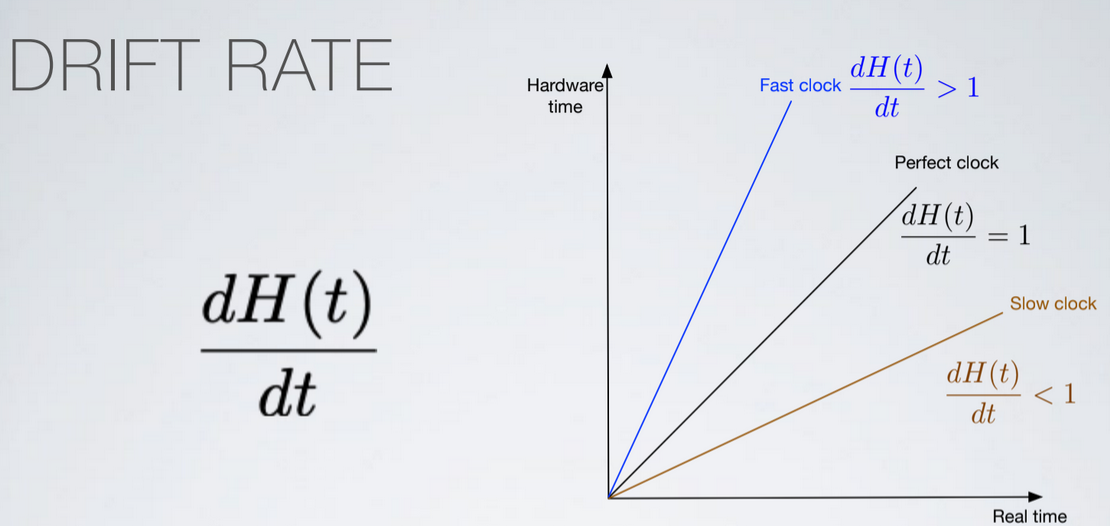
\includegraphics[scale=0.5]{img/clocks/dr.png}
\end{center}
To synchronize two clocks we have 2 strategies, either bring one in the future or bring it in the past by modifying beta, we never go into the past as we may have done something before the sync and it would cause confusion. We can however slow the clock that is in the future.
\begin{center}
    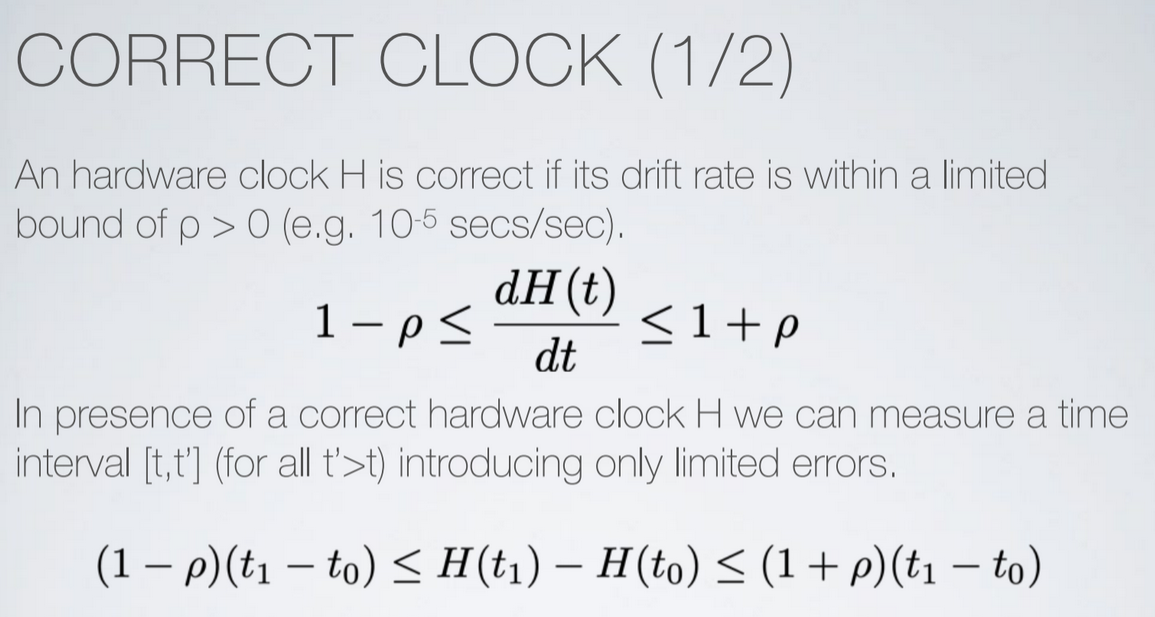
\includegraphics[scale=0.5]{img/clocks/cc1.png}
    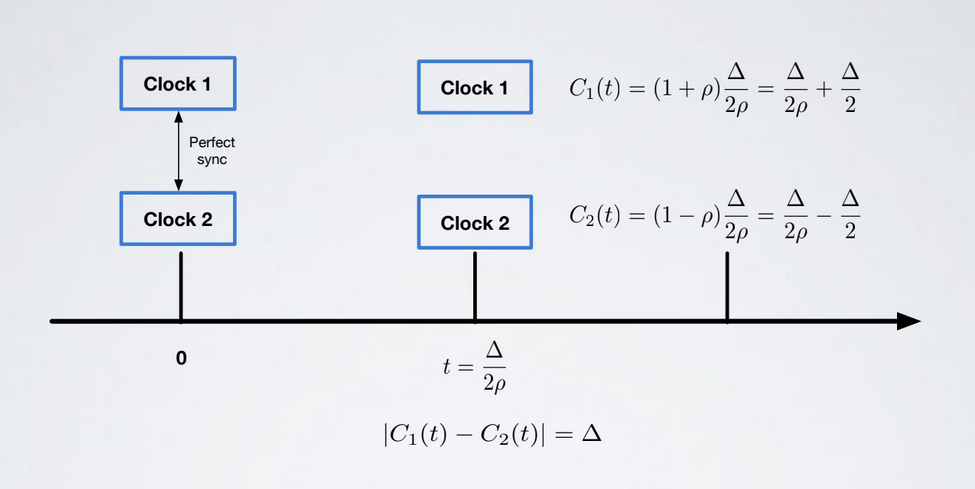
\includegraphics[scale=0.6]{img/clocks/cc2.png}
    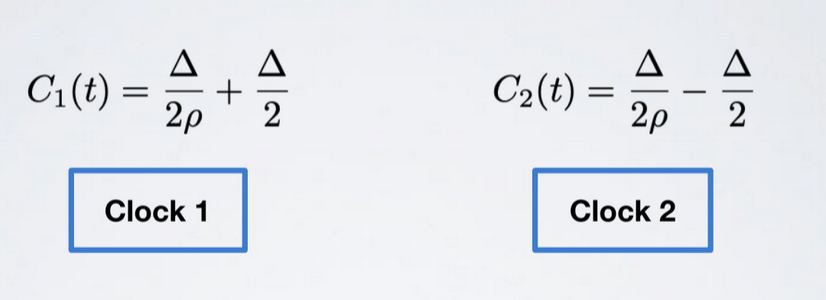
\includegraphics[scale=0.7]{img/clocks/cc3.png}
    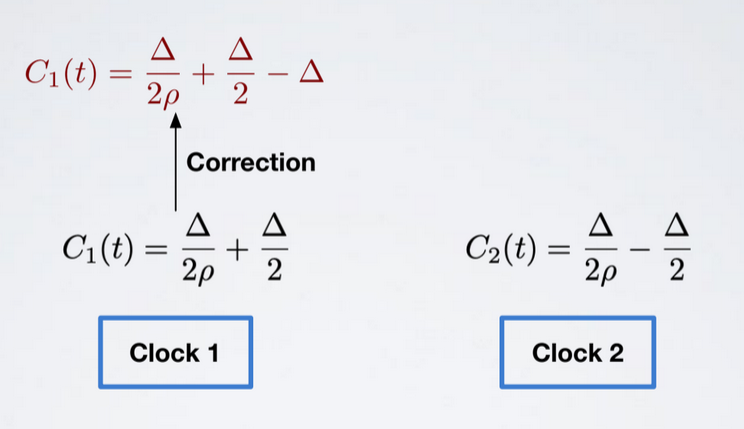
\includegraphics[scale=0.7]{img/clocks/cc4.png}
\end{center}
All software clocks have to be monotone:
$$ t' > t \implies C(t') > C(t)$$
So if real time t' is greater than t, we have that the software clocks reflect that, to actually reflect this, we cannot choose a value $\beta$ in the negatives, but rather
a value $\alpha$ that is $<$ 1 by \textit{masking oscillations} as well changing the value $\beta$.\\
When we synchronize with external time, we synchronize with UTC as it is the international standard and we'll synchronize via satellites.\\
We can define \textbf{external synchronization} when we synchro with UTC, so each process is synchronized with an authorative external source, this means that the difference between any computer and the external source is below a certain bound D.\\
If we don't synchro with the external world we are doing \textbf{Internal synchronization}, a set of processes is internally synchronized if the difference between their clocks is less than D. If we have external we also have internal.
\subsection{Algorithms for synchronization}
For external synchronization we have christian's algorithm, we utilize a Server S that receives a signal from an UTC source, works (probabilistically) in async systems, its based on RTTs, and only if RTTs are small and respect the required accuracy will the response be considered. We can also divide  to know the difference between when the server sent the info and when I received it, so just add $time\_ response + \frac{RTT}{2}$ but this assumes that RTT is symmetric.
Another problem is the fact that we have a single point of failure (server) in real life we just synchronize with multiple servers.
\begin{center}
    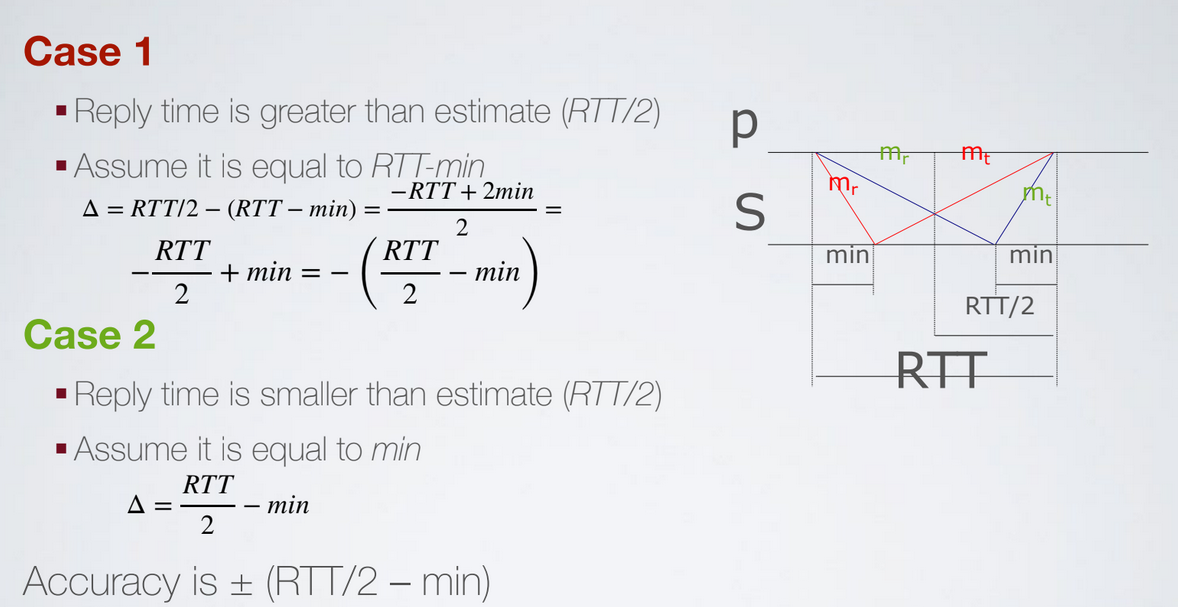
\includegraphics[scale=0.5]{img/synchro_algs/christian.png}
\end{center}
For internal clock synchronization we have the Berkley algorithm, in which we have a master/slave architecture,
where the master process $p_m$ sends a message with timestamp $t_1$ (local clock) to each process including itself, after that when each process receives a message from the master, it sends back a reply with a timestamp $t_2$ (local clock value), the master then receives the reply, reads it local clock and computes the difference between the clocks. We will then compute an average value of all non-faulty processes (difference is not more than a certain y) and the master will compute Deltas for each computer.\\
\\
Let's see an example:\\
We have the master, with a time of 3:05, then we have slave 1 with 2:55, then
slave 2 with 3:00 and slave 3 with 3:25. The master asks the time for everyone,
receiving the answers. The master will now compute the delta between the master
and itself, which is obviously zero, then He will do the same for $\Delta$M1 = -10, then
$\Delta$M2 = -5 and then $\Delta$M3 = 20. By using those quantities, we'll compute an
average difference, but before doing so the masters will remove processes who are
likely faulty, so processes who surpass a certain threshold. By setting the
threshold, for example, at 10, we will remove $\Delta$M3, because it's 20 $>$ 10. We will
now have that Avg = 0-10-5
3 = -5.
We'll tell anyone now that, in order to move to the correct value, the process will
have to move to $\Delta$Mi - Avg. For example, for the slave 1 he'll have to move to
-5 - (-10) = +5. The slave 2 will have to move of -5 - (-5) = 0. We compute
also for slave 3, by having -5 - 20 = -25. Also for the master, by having
-5 - 0 = -5. Each process will now be at 3:00.
\begin{center}
    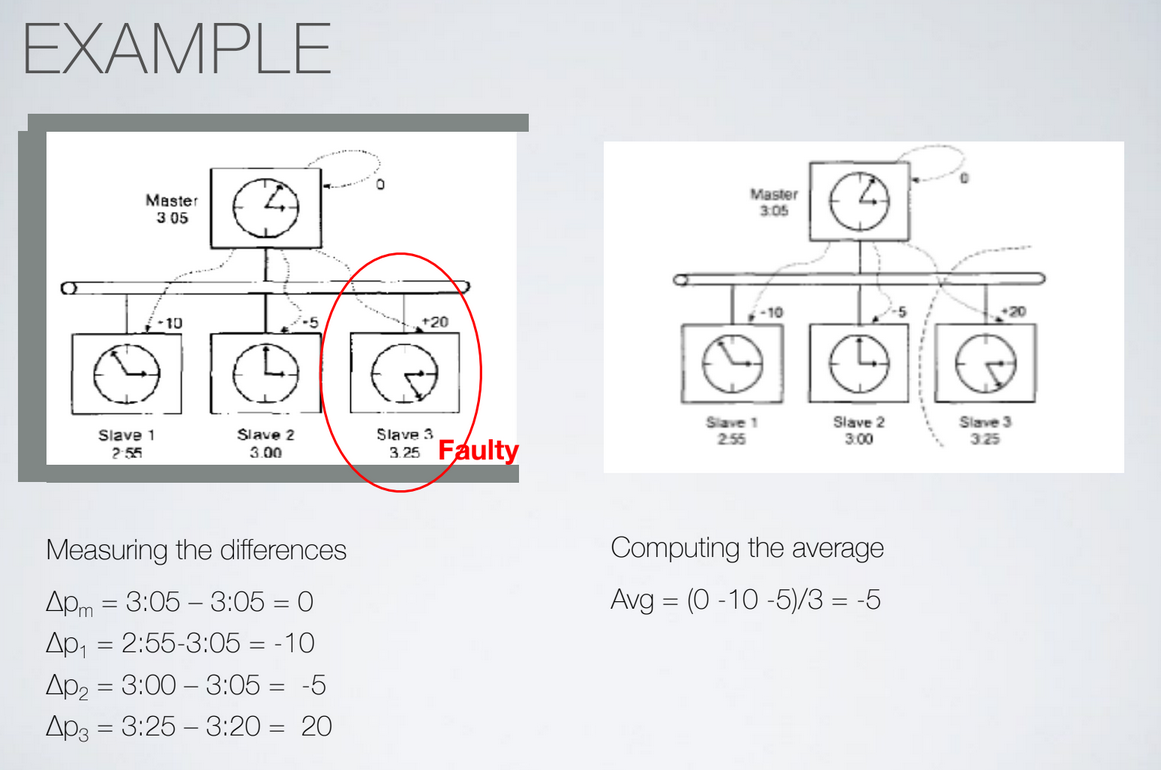
\includegraphics[scale=0.4]{img/synchro_algs/berk1.png}
    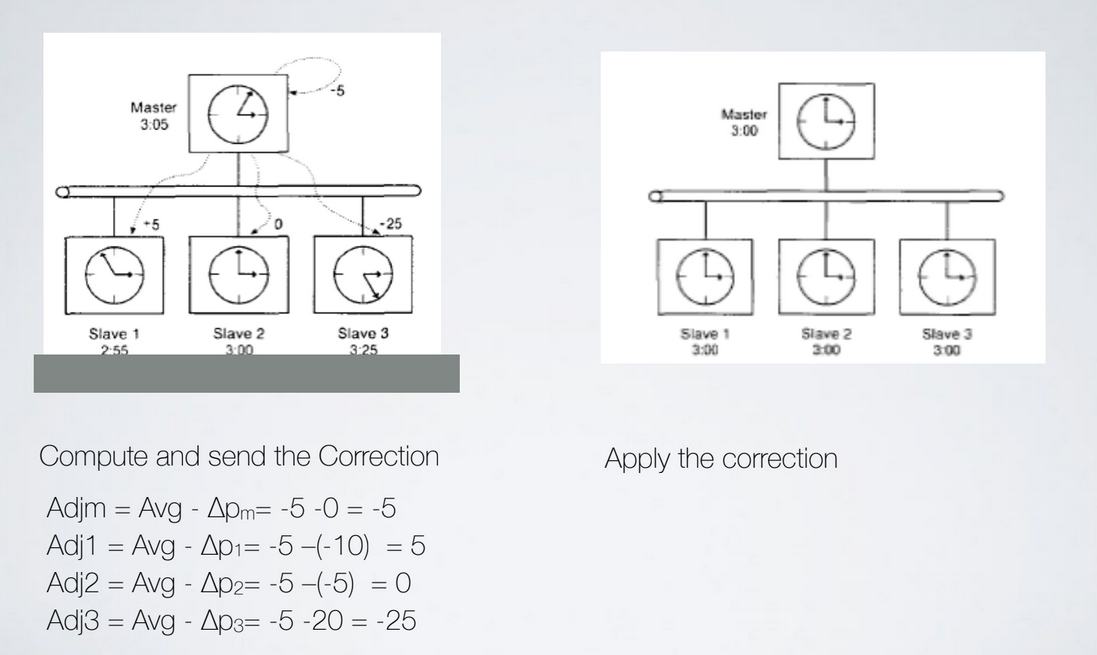
\includegraphics[scale=0.4]{img/synchro_algs/berk2.png}
\end{center}
For simplicity here we can go back in time, though in real life we should slow
down the clock.\\
The accuracy of Berkley depends on the maximum round trip time, as the master does not consider values associated with RTTs higher than a threshold, this algorithm is also not fault tolerant for the master, if the slaves are faulty the algorithm still works, if the master crashes, eventually a new one will be elected.\\\\
In real life we use \textbf{NTP} (Network Time Protocol), it synchronizes computers with
UTC.\\
The servers are organized in a hierarchy. The server at the top has the clock. The
second level (stratum) synchronize directly with server 1, with an algorithm
similar to Christian's one. The  third stratum  only synchronize with stratum 2.\\
We can
have more stratums, like 4 and so on. Error propagates with the descension of
stratum (so stratum 3, for example, will have a cumulative error of $e_1$ and $e_2$).\\
We
do so such that the bandwidth of the server 1 is not completely saturated.\\
Clock synchronization has a limit, we can do it only on synchronous system, we
have to have predictable delays in the channel.\\
Even on synchronized systems, we could have a problem with clocks, given by the
bounded accuracy. The problems take place when the bound of the error overlaps
with the bound of the error of another process, but not guarantee the order.
\begin{center}
    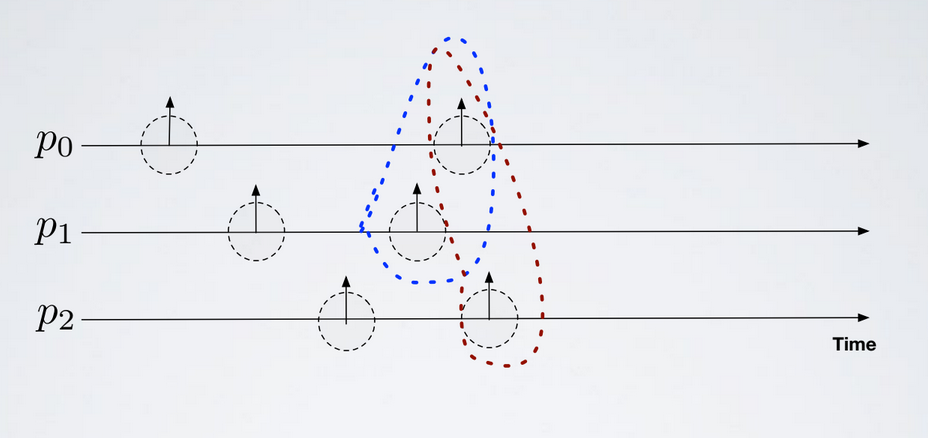
\includegraphics[scale=0.6]{img/synchro_algs/NTP.png}
\end{center}
\subsection{Logical Time}
Logical time is a concept of time we can implement also in asynchronous systems.
It takes care of the causal relationship between events. We'll talk about two
methods given by Scalar/Lamport's clocks, and then about Vector Clocks, used to
measure logical time. We'll also see Lamport's Mutual Exclusion algorithm.\\\\
Let's do an example.\\
Let's say we want to build a chat application. The easiest thing to do would be
using a server-client structure. If we are in a scenario with crash failures, if the
server dies the application stops working. Another way is not using a server,
i got
lost sorry.\\\\
Let's say we have a chat application with a specific pattern of messages. We have
Alice asking a question, then Mike responds, then Alice asks another question and
then another entity answers. This would be the real order of messages.\\
Because of the fact that the system is asynchronous, a broadcast message might
arrive with a certain delay to other entities.\\\\
Let's say that Bob, at a certain time t, only receives the messages from Mike and
Bob's supervisor, and not those from Alice. Bob would have a limited local view.
To avoid this kind of problem we have to formalize the concept of causality (the
messages of Mike, ecc are caused by Alice sending the first message).\\
The simple FIFO ordering, in this situation, will not help us. Our goal is to find a
way to timestamp an event, and to do that we have to formalize the concept of
causality, and then we timestamp events.\\\\
The definition of casual relationship was introduced by Lamport. We say that an
event happens before one another if there is a casual relationship between these
two.\\
Let's say that I have $p_0$, and two events happen on it, $e_0$ and then $e_1$. In this case
there is a casual relationship that $e_0$ happens before $e_1$ (we write it with an
arrow).\\
With condition B, let's say we have $e_1$ that's the sending of message m, $e_2$ the
receival. We say that $e_1$ happens obviously before $e_2$ (we received a message because
someone has sent it).\\
We can now define a partial ordering between events in the system, we introduce
three properties
\begin{center}
    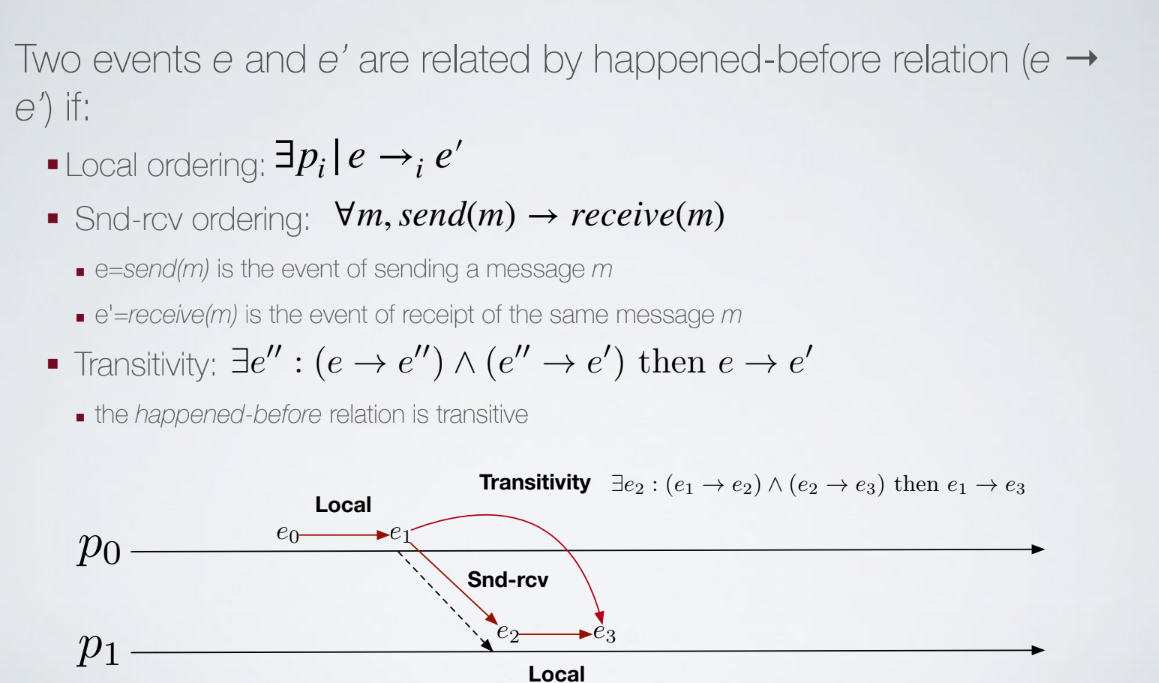
\includegraphics[scale=0.5]{img/logical time/properties.png}
\end{center}
The first property is the local ordering, (A) in the slides, and the second receive is
(B).
For the first, for example, we say that e and e' are related if a process $p_i$ exists by which $e \rightarrow_i e'$ (e is related with e' in $p_i$)\\
Then we have transitivity. This relationship (in the photo) is telling us that $e_3$
knows about $e_0$.\\\\
This relationship is partial, we could have events related by "happened before",\\
Let's say we have on $p_0$ another process $e_4$ happening. We say $e_3$ and $e_4$ are
concurrent. Two events are concurrent if they do not know about each other. The
only way to have them know is having a message from $p_0$ to $p_1$ or viceversa.
\begin{center}
    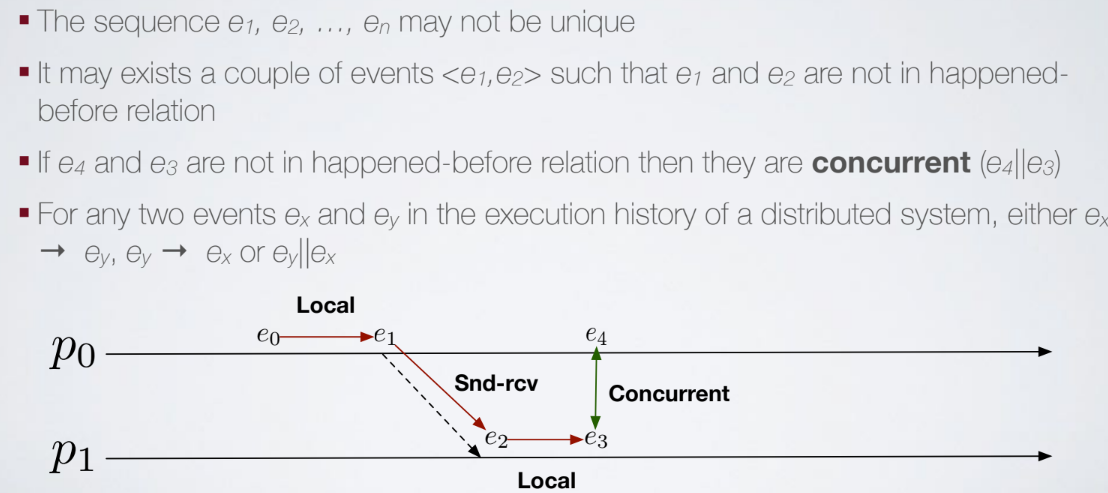
\includegraphics[scale=0.5]{img/logical time/hprel1.png}
    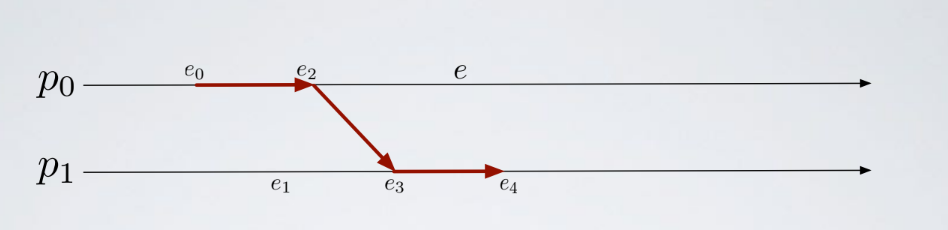
\includegraphics[scale=0.6]{img/logical time/hprel2.png}
    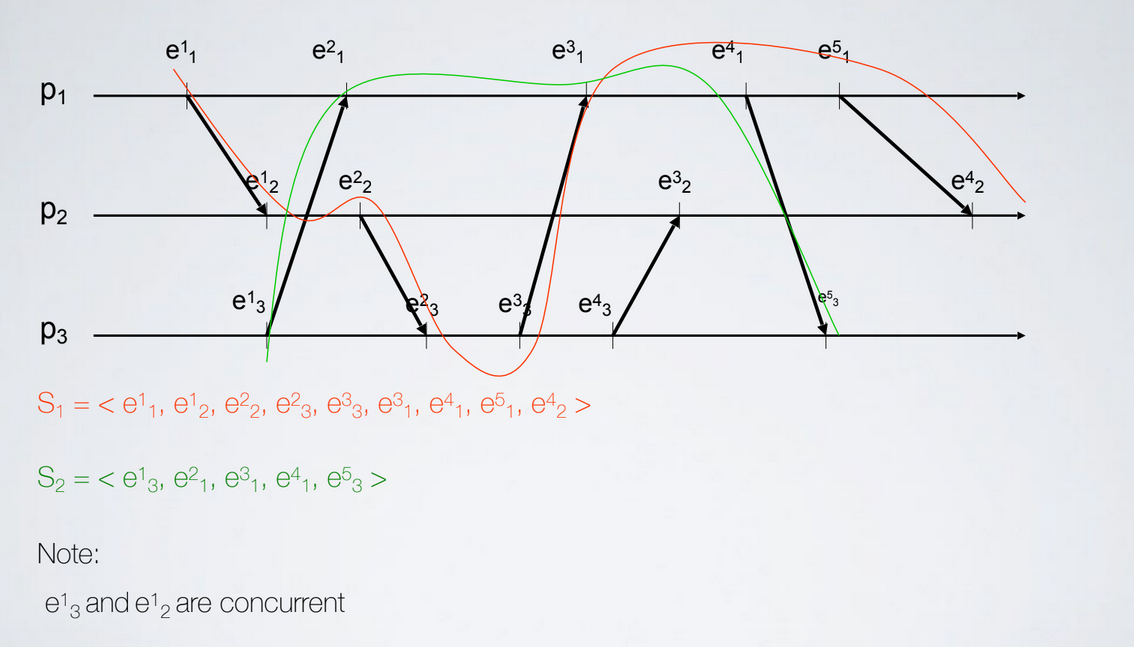
\includegraphics[scale=0.5]{img/logical time/ex1.png}
\end{center}
To see if two events are concurrent or not, we could try to find a path between
them.\\
Let us start with the first tool, the Logical Clock (Lamport's Clock).\\
We attach timestamp to each event, and this number will have a special property,
indicated as Li(e). We have that if e happens before e', then L(e) $<$ L(e'). (Only
works with $\implies$ , not with $\leftarrow$). If the logical clock of e is smaller than e', then this
doesn't imply that e has happened before e', they might be concurrent.\\
With the logical clock everyone starts with a counter Li, initially set to 0. We then
increase the counter, by following two rules:
\begin{itemize}
    \item when a local event happens, we increase the counter by  1
    \item when we send a message, we also increase the counter by 1. Along side sending the message, we also send the value of the counter ((m, 2) for example)
\end{itemize}
When I receive a message as process, we'll do a 1 + Max(L, L(m)) (maximum
between our logical clock and the value sent with the message), setting our counter
to that value.\\
We have to show that e → e' (e happens before e'), then L(e) $<$ L(e'). If e happens
before e', we have a path between e and e'. Whether the possibility, we increase by
at least one the value of the logical clock. Then if e happens before e', we'll have
that L(e') is greater at least by 1 than L(e).
\begin{center}
    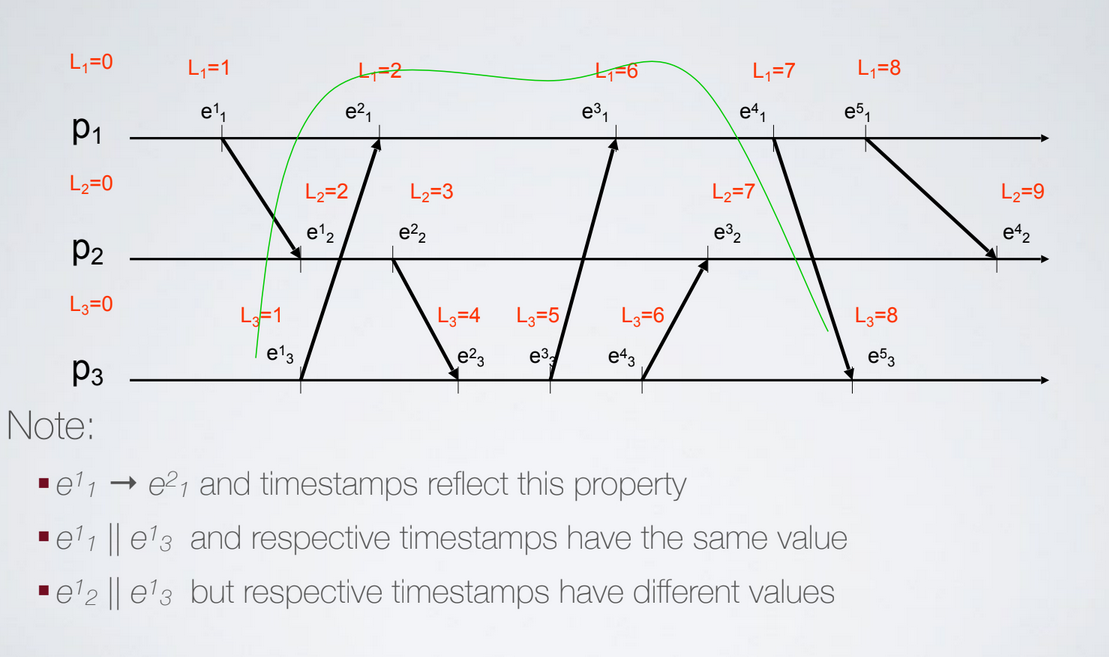
\includegraphics[scale=0.5]{img/logical time/ex2.png}
\end{center}
We would like to have now the $\iff$ for the relationship of local clock. There
exists Vector Clock, which allows us to design a system which has the other
direction of the property. We do not have a simple number, but a vector. By
comparing vectors, we'll be able to tell if an event happen before another.\\\\
As step 1 we construct this vector as a list of events, as step 2 we transform this
list of events in a vector. We attach then a data structure attached to an event,
which summarizes the history of the events.
\begin{center}
    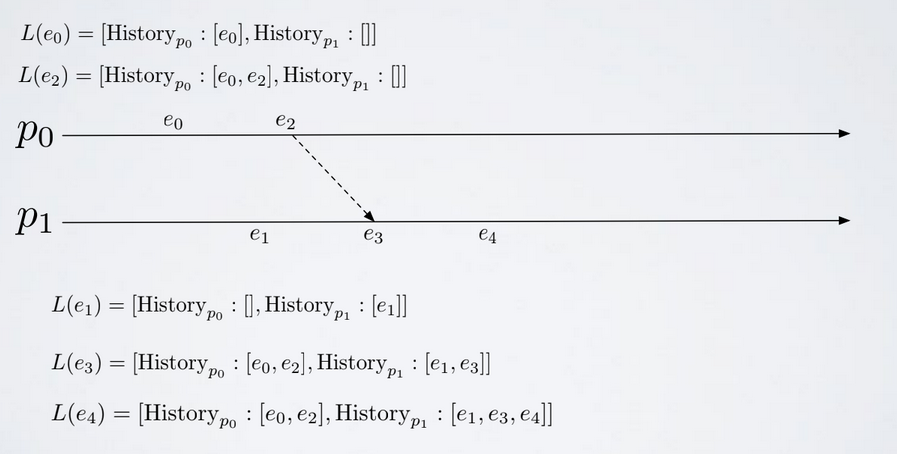
\includegraphics[scale=0.6]{img/logical time/ex3.png}
\end{center}
We'll have one entry (in the data structure) for each process.\\
At first the data structure will be [[], []] both for $p_0$ and $p_1$. When process zero
creates an event $e_0$, it's history will change. At this point we still do not know
nothing about $e_1$. Same goes for $e_1$ for $p_1$.\\
The local event is trivial, the "problem" is when we send a message. The message
will include the history of $p_0$ and $p_1$ (which at $e_2$ it's still empty). When $p_1$ receives
the message, he will now know the history of $p_0$ and its as well. We'll fill the
history of $p_0$ with the longest one (received with the message), and the history of
$p_1$ will be made by $e_1$ and $e_3$.\\
What we are doing is that we are constructing the view of the process. Now, how
do we compare data structures? We say that L(e) $<$ L(e') if, for each location of
the history, the list is smaller than the other. As example of history of $e_0$ and $e_3$.
Some data structures are not comparable, for example $e_0$ and $e_1$, as we have
[[$e_0$], []] for $e_0$ and [[], [$e_1$]]. For the first location $p_0$ is winning, but then for the
second one $p_1$ is winning, they are not comparable. This happens because the
events are concurrent.
Let's see the proof.
We have to show that if e → e' then L(e) $<$ L(e') (data structure of e is contained
in e''s one). If e happens before e', then there is a path between e and e', then the
data structure at e' will contain the one of e.
How to show the other direction? If the data structure of e is smaller than e', then
e → e'. If the data structure of e is less than e', then L(e) is contained in L(e'),
then all events happened at e then they are contained in L(e'). Because of the fact
that e is contained also in L(e'), then there must be a path that somehow has
connected e to e', then e → e'.\\
This data structure captures causality.\\
What are the disadvantages of using this data structure? The use of a large
amount of memory for a lot of events. How do we get something more compact?
Let's say that on my system I find two events, e and e'. I examine the data
structure of e and e' and I find that, for a certain location x in the history, I find
something similar.\\
To have something different would be impossible (like in the slide's example)\\
\begin{center}
    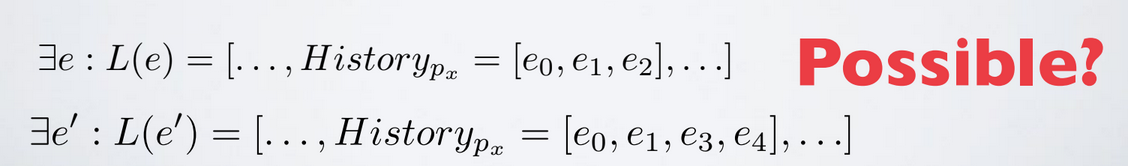
\includegraphics[scale=0.5]{img/logical time/ex4.png}
\end{center}
The only one who can append something at the history of px is px itself, so the
last event can't be different.\\
What matters is not the content of the list, but the size of the list. We can then
compress the data structure by just using the size of the list.\\
So at first we start with a vector for all zeros, having empty lists for each process.\\
Let's say we are p1 and we create a new event, then I increase the value of +1 for
the size of p1. When another process receives a message, it compares the elements
between the lists and take the maximum.\\
We can say that one vector is less than the other (V (e) $<$ V(e')) if all components
are $\leq$ and there is one component who is strictly less.
\end{document}